\chapter{固定拓扑持续学习的统一闭环}

\begin{chapteroverviewbox}
本章完成第二编“AgentOS 原理论”的第一次总收束。此前各章分别建立了三相记忆
$h$--$E$--$\Theta$、自我慢变量 $\Psi$、生命周期生成吸引子 $\Omega$、工作记忆有限容量约束、
SPC 自我状态估计、AHC 内稳态调制、TCE 认知动力学控制、CCM 运行复杂度治理、
Scheduler 调度、Boundary 准入与边界控制、Offloading 外部承载，以及连续动力学与离散治理等结构。
如果这些组件仅被并列描述，它们仍然只是一个模块集合；本章的任务，是把它们重新写成一个具有明确
状态变量、时间尺度、反馈方向、控制目标和稳定性条件的统一动力系统，并回答一个关键问题：

\begin{statementbox}
在功能拓扑保持基本固定的条件下，一个 Agent 能否仍然实现真正意义上的持续学习、
\end{statementbox}

\begin{statementbox}
能力成长、身份连续、自我调节以及对未来自身的递归影响？
\end{statementbox}

本章给出的回答是：在相当大的能力范围内，可以。固定拓扑并不等于固定状态、固定记忆、固定策略或固定自我。
只要系统允许认知结构在既定功能通路中改变表示、激活位置、时间尺度、记忆深度和内外承载方式，并允许
慢变量根据长期经验持续更新，那么系统仍然可以形成显著的生命周期成长。其本质并不是
$\mathcal{T}$ 本身发生改变，而是在固定的功能拓扑 $\mathcal{T}_0$ 上发生持续的
\emph{state dynamics、memory dynamics、structural consolidation、self dynamics、
control dynamics 与 carrier migration}。

因此，本章研究的是：

\begin{statementbox}
Dynamics on a Fixed Topology
\end{statementbox}

而不是后续意义上的：

\begin{statementbox}
Dynamics of the Topology Itself.
\end{statementbox}

这一界限非常重要。它使我们能够首先回答“一个持续主体怎样活着、学习和成长”，再讨论更强的
“一个持续主体怎样修改承载自身认知的功能组织”。本章同时也是后续 AgentOS 工程实现的理论基线：
任何未来允许拓扑自重组的系统，都首先必须能够在拓扑不变时稳定运行，否则所谓结构可塑性只会把
运行时不稳定进一步放大。
\end{chapteroverviewbox}

\begin{figure}[htbp]
\centering
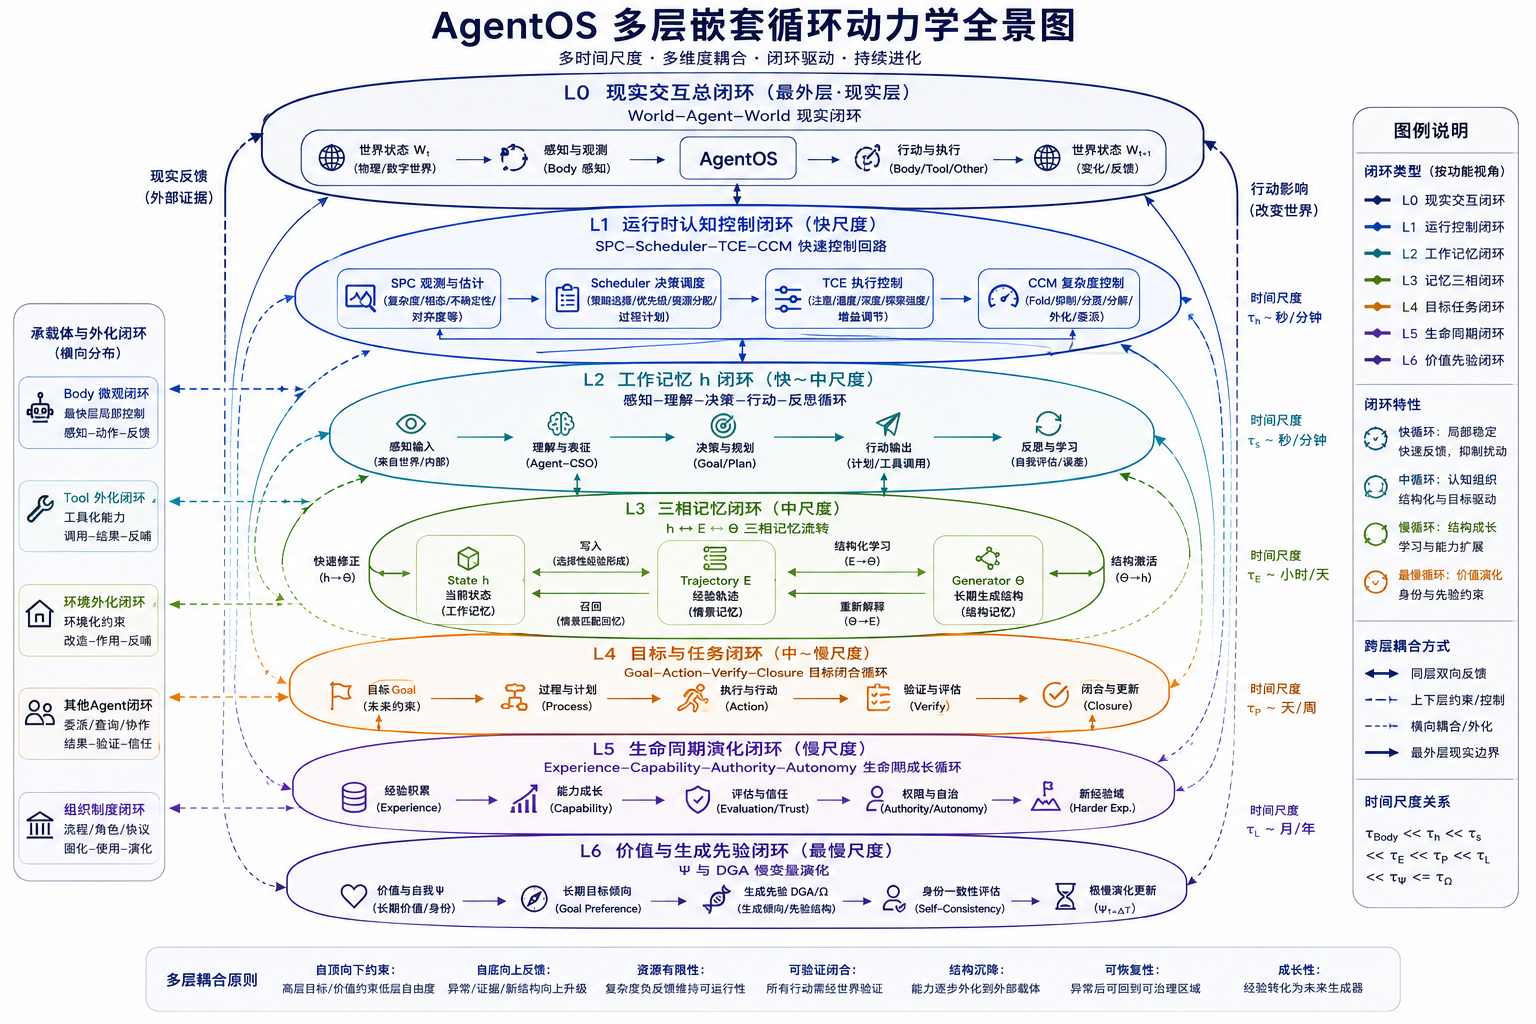
\includegraphics[width=.9\textwidth,height=.38\textheight,keepaspectratio]{images/agentos-continuous-learning-architecture.png}
\caption{固定拓扑持续学习的统一闭环}
\end{figure}
\begin{introduction}[本章导航]
  \item 固定拓扑持续学习的严格定义
  \item 生命周期统一状态空间与核心闭环
  \item 有限工作记忆的可运行性条件
  \item 自我、DGA 与身份连续性
\end{introduction}

\section{固定拓扑持续学习问题的严格定义}

我们首先需要澄清“固定拓扑”究竟意味着什么。若把固定拓扑错误理解成“系统内部一切都不允许变化”，那么持续学习当然不可能发生；但这并不是本书所讨论的对象。这里所谓固定拓扑，是指 AgentOS 在一个给定生命周期阶段内，其主要功能节点及其允许发生作用的连接关系保持不变。设 AgentOS 的功能图为

\[
\mathcal{G}_{F}
=
(V_F,E_F,\mathcal{L}),
\]

其中 $V_F$ 表示功能节点集合，$E_F$ 表示允许的信息、控制与记忆耦合通道，$\mathcal{L}$ 表示由这些节点和边构成的闭环集合。固定拓扑条件可以形式化为

\[
\operatorname{supp}A_F(t)
=
\operatorname{supp}A_F(0),
\qquad
t\in[0,T_L],
\]

其中 $A_F$ 是功能图的邻接关系，$\operatorname{supp}$ 表示哪些边实际存在。这个条件约束的是“哪些功能原则上能够长期直接耦合”，而不是说连接上的信号强度、节点内部状态、参数、激活模式或者当前承载的认知结构都必须保持不变。

因此，一个更准确的固定拓扑 AgentOS 应被写成

\begin{statementbox}
\centering
\adjustbox{max width=.96\linewidth}{\(\displaystyle \mathcal{T}(t)=\mathcal{T}_0,
\qquad
X(t),\Theta(t),\Psi(t),\Omega(t),\mu_t
\ \text{均可变化}.\)}
\end{statementbox}

这里 $\mathcal{T}_0$ 是固定功能拓扑，而 $X(t)$ 表示快速运行状态，$\Theta$ 表示长期生成结构，$\Psi$ 表示自我与身份慢变量，$\Omega$ 表示生命周期生成倾向，$\mu_t$ 则描述当前认知结构由哪些功能节点承载。换言之，固定的是“道路网的基本存在关系”，而不是道路上正在运输什么、交通流量多大、哪些道路当前被优先使用，以及货物被存放在何处。

这一点可以用 CSO 理论进一步澄清。若某一认知结构 $C$ 在 Agent 内部具有具体承载：

\[
AgentCSO_A(C,t)
=
(C,R_t,F_t,\tau_t,B_t,S_t),
\]

那么固定拓扑并不要求

\[
R_t,\;F_t,\;\tau_t,\;B_t,\;S_t
\]

全部固定。相反，持续学习恰恰体现在这些变量的变化之中。例如，一项新任务最初可能以显式结构存在于 $h$ 中，需要高强度推理；经过反复经验以后，它可以在 $E$ 中形成稳定轨迹，进一步被 $\Theta$ 抽象为规律或技能，最后通过 Offloading 或技能编译转移到工具、程序或者 Body 的局部闭环中。只要这些迁移使用的功能路径原本已经存在，就没有发生拓扑改变，却已经发生了非常实质性的学习。

因此，我们需要区分三个层次：

\[
\boxed{
\text{State Change}
<
\text{Structural Change}
<
\text{Topological Change}.
}
\]

状态变化是当前运行内容变化；结构变化是记忆、表示、自我、策略或承载关系变化；拓扑变化则要求长期功能关系本身被新增、删除、拆分或重组。本章专门研究前两个层级。

从动力系统角度，可以把固定拓扑 Agent 写成一个参数与慢变量可变的混合系统：

\[
\dot{x}
=
f_{\mathcal{T}_0}
\left(
x,
z,
u,
w
\right),
\]

\[
z_{k+1}
=
g_{\mathcal{T}_0}
\left(
z_k,
\mathcal{E}_k,
x_{[k]}
\right),
\]

其中 $x$ 是快速连续状态，$z$ 是较慢结构状态，$u$ 是内部控制信号，$w$ 是环境扰动，$\mathcal{E}_k$ 是被选择并固化的经历。函数族由 $\mathcal{T}_0$ 限定，但其内部状态和参数持续改变。这与控制理论中的固定系统结构加自适应参数、计算机系统中的固定指令架构加持续状态变化，以及认知科学中的稳定功能系统加记忆巩固存在形式上的相似性。

因此，本章真正研究的不是“一个静态 Agent 如何保存更多数据”，而是：

\begin{statementbox}
一个保持主体组织骨架不变的系统，如何通过内部多时间尺度状态迁移形成生命周期成长。
\end{statementbox}

这也解释了为什么固定拓扑并非低级阶段。恰恰相反，它是身份连续、安全验证和长期稳定性研究所必需的理论基准。如果一个 Agent 连在主要功能拓扑保持不变时都无法形成稳定自我、可靠记忆和可治理学习，那么允许它动态修改拓扑不会创造成熟智能，只会增加新的自由度和新的失稳渠道。

\section{统一状态空间：从当前认知到生命周期慢变量}

为了描述固定拓扑 AgentOS 的持续学习，我们需要把此前分散的状态统一到同一个多时间尺度状态空间中。一个最小而又足够完整的生命周期状态可以写成

\[
\boxed{
\mathcal{X}_A(t)
=
\left[
h_t,
E_t,
\Theta_t,
a_t,
\Psi_t,
\Omega_t,
G_t,
Q_t
\right].
}
\]

其中，$h_t$ 是当前工作记忆状态，$E_t$ 是情景与经验轨迹集合，$\Theta_t$ 是长期生成结构，$a_t$ 是 AHC 的内稳态与情感样调制状态，$\Psi_t$ 是身份、自我和价值相关慢变量，$\Omega_t$ 是 DGA 所代表的生命周期生成吸引子，$G_t$ 是当前及中长期目标结构，$Q_t$ 则表示离散治理状态，例如任务权限、运行模式、恢复点、安全等级以及当前哪些修改是被允许的。

这个状态向量并不意味着所有变量都以同样的时间分辨率更新。恰恰相反，AgentOS 的核心是时间尺度分离：

\[
\boxed{
\tau_h
\ll
\tau_E
\ll
\tau_\Theta
\ll
\tau_\Psi
\ll
\tau_\Omega.
}
\]

AHC 的典型时间尺度通常位于快速认知与较慢经验之间，而 Scheduler、SPC、TCE、CCM 等运行时控制过程主要作用在 $h$ 附近的快时间尺度。由此可以构造一个快---慢系统：

\[
\epsilon_1\dot{h}
=
F_h
(h,E,\Theta,a,\Psi,G,u,w),
\]

\[
\epsilon_2\dot{a}
=
F_a
(a,FCS,h,\Psi),
\]

\[
\dot{E}
=
F_E(E,h,a,\Psi),
\]

\[
\delta_\Theta\dot{\Theta}
=
F_\Theta(\Theta,E,\varepsilon),
\]

\[
\delta_\Psi\dot{\Psi}
=
F_\Psi(\Psi,\Theta,E,\mathcal{R}),
\]

\[
\delta_\Omega\dot{\Omega}
=
F_\Omega(\Omega,\Psi,\Theta,\mathcal{H}),
\]

并满足

\[
\epsilon_1
<
\epsilon_2
\ll
1,
\qquad
\delta_\Omega
\ll
\delta_\Psi
\ll
\delta_\Theta.
\]

这里的目的不是宣称真实 Agent 必须使用这些具体微分方程，而是明确一个原则：\emph{越接近当前决策的变量越快，越接近身份、生成倾向和生命周期方向性的变量越慢。} 这种时间尺度排序正是稳定性与可塑性能够共存的根本来源。

如果所有变量都以 $h$ 的速度变化，那么系统虽然极度可塑，却没有身份；如果所有变量都以 $\Omega$ 的速度变化，那么系统虽然稳定，却无法适应。持续智能需要的是：

\[
\boxed{
FastPlasticity
+
SlowContinuity.
}
\]

这也解释了为什么三相记忆不能被理解成三个数据库。$h$ 是系统的实时显式表面；$E$ 是被选择后的轨迹结构；$\Theta$ 是对经验进行压缩后能够重新生成预测、规则和技能的结构。它们不是三个互不关联的容器，而是三个不同动力时间尺度上的同一认知结构生命周期。

对于某一 CSO $C$，我们甚至可以写出其典型迁移轨迹：

\[
C_h
\rightarrow
C_E
\rightarrow
C_\Theta,
\]

其中

\[
\tau(C_h)
<
\tau(C_E)
<
\tau(C_\Theta).
\]

但这一方向并非不可逆。在新的现实扰动出现时：

\[
C_\Theta
\rightarrow
C_h
\]

意味着长期结构重新被激活；若旧结构不能解释现实，则：

\[
C_h
\rightarrow
C_E'
\rightarrow
C_\Theta'
\]

意味着经历对结构发生重新塑造。由此，持续学习不是简单的“写入长期记忆”，而是结构在多个时间尺度之间循环。

身份连续性则建立在更慢的 $\Psi$ 与 $\Omega$ 上。我们可以把 $\Psi$ 看成对大量经验和长期结构进行进一步低频整合后的自我约束：

\[
\Psi_{k+1}
=
\Psi_k
+
\eta_\Psi
\mathcal{F}_\Psi
(
\Theta_k,
E_{[k-m:k]},
R_k
),
\]

其中

\[
\eta_\Psi
\ll
\eta_\Theta.
\]

同理：

\[
\Omega_{k+1}
=
\Omega_k
+
\eta_\Omega
\mathcal{F}_\Omega
(
\Psi_k,
\Theta_k,
G_k,
\mathcal{H}_k
),
\qquad
\eta_\Omega
\ll
\eta_\Psi.
\]

因此，一次失败可以迅速改变 $h$；连续多次失败可能改变 $E$ 对某类任务的经验分布；长期稳定的失败模式才有资格显著修改 $\Theta$；而只有跨时间、多情境、持续一致的结构证据，才应对 $\Psi$ 甚至 $\Omega$ 产生明显影响。

这一多尺度状态空间是整个固定拓扑持续学习理论的核心，因为它证明了一个重要事实：\emph{功能拓扑不变化，并不意味着生命周期状态空间没有深度。} 一个拓扑完全不变的系统，只要拥有足够丰富的多尺度慢变量，同样能够在很长时间中形成明显不同的“早期自我”“成熟自我”和“未来倾向”。

\section{核心生命周期闭环：从现实扰动到未来选择}

在统一状态空间基础上，我们现在可以把此前所有模块重新组织成一个完整闭环。一个真实 Agent 的学习不是从“训练数据”开始，而是从现实中的扰动、事件、需求和自身状态变化开始。设环境状态为 $W_t$，经过当前观察界面形成对现实的有效输入 $O_t$。在不展开 Body Runtime 的情况下，可以把进入 AgentOS 内核的外部证据抽象为

\[
y_t
=
\mathcal{O}(W_t,B_t),
\]

其中 $B_t$ 表示当前感知与行动边界。

真正进入工作记忆的并不是全部 $y_t$，而是经过 Boundary、Scheduler 和 CCM 共同筛选后的有限结构：

\[
h_t
=
\mathcal{A}
\left(
y_t,
E_t,
\Theta_t,
\Psi_t,
G_t;
Bnd_t,
Sch_t,
CCM_t
\right),
\]

其中 $\mathcal{A}$ 表示准入与激活过程。于是当前显式认知本身已经是一个高度选择性的结果，而不是原始世界的复制。

随后 SPC 对当前内部动态形成估计：

\[
\hat{s}^{self}_t
=
SPC
\left(
h_t,E_t,\Theta_t,\Psi_t,a_t
\right).
\]

这里特别需要强调：

\[
\boxed{
\hat{s}^{self}_t
\neq
s^{self}_t.
}
\]

Agent 对自身的认识始终是估计，而不是透明访问。SPC 的作用恰恰是把分布式、部分不可见并具有时间滞后的内部状态压缩成一个能够进入当前认知过程的自状态表示。

AHC 接收该估计以及与身体、资源、风险、社会和任务相关的连续信号，并产生较平滑的调制状态：

\[
a_{t+1}
=
\mathcal{H}
\left(
a_t,
\hat{s}^{self}_t,
m_t
\right),
\]

其中 $m_t$ 是内稳态与影响信号。随后 TCE 根据当前认知状态、自我状态、AHC、目标、$\Psi$ 与 $\Omega$ 生成认知控制：

\[
u^{TCE}_t
=
\pi_{TCE}
\left(
h_t,
\hat{s}^{self}_t,
a_t,
G_t,
\Psi_t,
\Omega_t
\right).
\]

该控制不必直接指定下一条语言 token，而是调节探索程度、认知温度、注意范围、推理深度、保守程度、并发强度、记忆召回以及状态转换倾向。

经过一个或者多个快速循环后，Agent 产生行动 $u^{act}_t$，行动重新进入世界：

\[
W_{t+1}
=
F_W(W_t,u^{act}_t,\xi_t),
\]

其中 $\xi_t$ 表示不可控现实扰动。新的世界状态重新产生观测，从而形成真正闭合的：

\begin{statementbox}
\centering
\adjustbox{max width=.96\linewidth}{\(\displaystyle World
\rightarrow
Agent
\rightarrow
Action
\rightarrow
World.\)}
\end{statementbox}

但是，若闭环仅止于这里，系统只具有在线控制，而不是生命周期学习。持续学习要求当前过程被选择性写入 $E$：

\[
E_{t+1}
=
\mathcal{U}_E
\left(
E_t,
h_{[t_0:t_1]},
a_{[t_0:t_1]},
r_{[t_0:t_1]},
\Psi_t
\right),
\]

其中 $r$ 表示现实反馈、成功失败、预测残差等。被反复观察到的经验模式进一步形成：

\[
\Theta_{k+1}
=
\mathcal{U}_\Theta
(
\Theta_k,
E_{[k-m:k]}
).
\]

更慢尺度上：

\[
\Psi_{n+1}
=
\mathcal{U}_\Psi
(
\Psi_n,
\Theta_{[n-p:n]},
E_{[n-p:n]}
),
\]

而生命周期生成倾向则满足：

\[
\Omega_{q+1}
=
\mathcal{U}_\Omega
(
\Omega_q,
\Psi_{[q-r:q]},
\Theta_{[q-r:q]},
G_{[q-r:q]}
).
\]

最终，新的 $\Psi$ 与 $\Omega$ 又改变未来目标与选择：

\[
G_{t+\Delta}
=
\mathcal{G}
(
W_{t+\Delta},
\Theta,
\Psi,
\Omega
),
\]

\[
Choice_{t+\Delta}
=
\pi
(
h,
G,
\Theta,
\Psi,
\Omega
).
\]

于是整个闭环应当写成：

\begin{statementbox}
\centering
\adjustbox{max width=.96\linewidth}{\(\displaystyle World
\rightarrow
h
\rightarrow
SPC
\rightarrow
AHC/TCE
\rightarrow
Action
\rightarrow
World'
\rightarrow
E
\rightarrow
\Theta
\rightarrow
\Psi
\rightarrow
\Omega
\rightarrow
FutureGoal
\rightarrow
FutureChoice.\)}
\end{statementbox}

这就是固定拓扑 AgentOS 的生命周期学习闭环。它最重要的含义是：\emph{当前行为不仅改变世界，也改变未来做出行为的自己。}

因此，学习不再是一个独立于运行过程的后台函数，而成为运行本身的时间积分。今天的一次选择通过现实形成经历，经历进入 E，长期积累形成 $\Theta$，结构进一步影响 $\Psi$ 和 $\Omega$，最终改变未来 Agent 面对类似世界时的目标、注意、风险评价和行动方式。于是一个持续 Agent 的“过去”具有真实因果力量。

\section{有限工作记忆与可运行性的负反馈条件}

上述生命周期闭环只有在系统能够持续保持可运行状态时才具有意义。持续学习首先不是“学习得更多”，而是“在不断增加经验的情况下仍然不让当前认知系统崩溃”。这正是工作记忆有限容量定理在统一闭环中的位置。

设当前工作记忆中存在 $n_t$ 个活跃认知结构，每一个结构的有效处理负载为 $c_i(t)$，其当前全局资源权重为 $w_i(t)$，则可定义运行复杂度：

\[
C_{\mathrm{run}}(t)
=
\sum_{i=1}^{n_t}
w_i(t)c_i(t),
\qquad
\sum_iw_i(t)\leq 1.
\]

固定拓扑 AgentOS 必须维持：

\[
\boxed{
C_{\mathrm{run}}(t)
\leq
C_{\max}(W)
}
\]

至少在绝大多数正常运行区间内成立。这里的 $W$ 并不只是 token window，而是整个工作记忆能够同时保持相互关系、冲突约束、当前目标和行动计划的有效相干容量。

当

\[
C_{\mathrm{run}}(t)
>
C_{\max}(W),
\]

系统可能进入：

\[
\text{遗漏}
\rightarrow
\text{冲突}
\rightarrow
\text{推理链破裂}
\rightarrow
\text{错误率上升}
\rightarrow
\text{运行相态失稳}.
\]

因此，CCM、Scheduler、Boundary 和 Offloading 并不是四个附属模块，而是有限工作记忆条件下维持长期主体存在的必要负反馈结构。

我们可以把四者的联合控制写成：

\[
u^{gov}_t
=
\left[
u^{CCM}_t,
u^{Sch}_t,
u^{Bnd}_t,
u^{Off}_t
\right].
\]

CCM 首先估计：

\[
\hat{C}_{\mathrm{run}}(t),
\qquad
\widehat{\dot C}_{\mathrm{run}}(t),
\]

不仅判断当前是否超载，还预测未来是否即将进入危险区。若检测到：

\[
\hat C_{\mathrm{run}}
+
\lambda
\widehat{\dot C}_{\mathrm{run}}
>
C_{\mathrm{safe}},
\]

系统就不应等待彻底过载之后再清理，而应提前采取结构治理动作。

Scheduler 回答的是：

\begin{statementbox}
当前有限资源应该给谁？
\end{statementbox}

它对 Goal、Task、Memory Retrieval、Tool、Reflection 等竞争过程进行优先级调度。CCM 回答的则是：

\begin{statementbox}
当前进入运行区的结构怎样保持在可治理范围内？
\end{statementbox}

Boundary 更进一步回答：

\begin{statementbox}
什么根本不应该进入这一轮全局认知？
\end{statementbox}

Offloading 则回答：

\begin{statementbox}
哪些结构不应该继续由昂贵的当前认知承载？
\end{statementbox}

因此可以把四者理解成四道不同位置的负反馈：

\begin{statementbox}
\centering
\adjustbox{max width=.96\linewidth}{\(\displaystyle Boundary
\rightarrow
Scheduler
\rightarrow
CCM
\rightarrow
Offloading.\)}
\end{statementbox}

Boundary 是入口控制；Scheduler 是竞争控制；CCM 是运行区稳定控制；Offloading 是结构释放和承载迁移。

在原来的复杂度治理语言中，我们曾将其概括为五类动作：

\begin{conclusion}
截流、压缩、时序展开、迁移、重构.
\end{conclusion}

在新的 CSO 语言下，可以更准确地写成：

\[
\fitdisplay{
Admission,
\quad
Compression,
\quad
Temporalization,
\quad
CarrierMigration,
\quad
RepresentationReorganization.
}
\]

例如，一个过大的问题不必一次塞入 $h$，而可以被展开成：

\[
C
\rightarrow
\{C_1,C_2,\ldots,C_m\},
\]

再按时间顺序执行：

\[
C_1
\rightarrow
C_2
\rightarrow
\cdots
\rightarrow
C_m.
\]

这实际上把空间同时复杂度转换成时间复杂度。另一些反复出现的结构则可以：

\[
h
\rightarrow
Skill,
\quad
h
\rightarrow
File,
\quad
h
\rightarrow
Tool,
\quad
h
\rightarrow
Environment.
\]

因此成熟智能的标志不是 $h$ 越来越大，而是：

\begin{statementbox}
\centering
\adjustbox{max width=.96\linewidth}{\(\displaystyle \frac{\text{需要全局显式认知的结构量}}
{\text{系统成功完成的总结构处理量}}
\downarrow.\)}
\end{statementbox}

也就是说，持续学习真正成功时，系统并不是把越来越多东西长期堆积在当前思维里，而是越来越善于让已经掌握的结构离开昂贵的显式认知区域。

\section{三相记忆循环如何在固定拓扑中实现结构成长}

现在我们进一步分析：如果功能拓扑不变化，Agent 的“成长”究竟发生在哪里？答案首先发生在 $h$、$E$ 与 $\Theta$ 之间的结构循环中。

我们可以把三相记忆写成三个具有不同结构自由度的状态空间：

\[
h_t\in\mathcal{H},
\qquad
E_t\in\mathcal{E},
\qquad
\Theta_t\in\mathcal{\Theta}.
\]

$h$ 保存当前需要显式操作的高活动结构；$E$ 保存带有时间、情境、结果和自我归属的轨迹；$\Theta$ 则保存跨经历压缩后仍然有效的稳定结构。持续学习不是把同一份数据复制三遍，而是三个空间之间发生信息形式变化。

首先是：

\[
h\rightarrow E.
\]

不是所有进入 $h$ 的内容都值得成为经历。写入概率可以概念化为：

\[
\fitdisplay{
P(write_E\mid x)
=
\sigma
\left(
\alpha_1 Novelty
+
\alpha_2 GoalRelevance
+
\alpha_3 PredictionError
+
\alpha_4 AHCIntensity
+
\alpha_5 SelfRelevance
\right).
}
\]

因此 E 是选择性历史，而不是录像机。Agent 的人生史本身就带有目标、自我与调制偏差。

随后：

\[
E\rightarrow\Theta
\]

意味着经验中的偶然细节被进一步压缩：

\[
\Theta'
=
\arg\min_{\Theta}
\left[
L_{\mathrm{pred}}
(E\mid\Theta)
+
\lambda_1C(\Theta)
+
\lambda_2L_{\mathrm{inconsistency}}
\right].
\]

这个表达式说明，长期结构需要在解释经验、结构简洁性和内部一致性之间取得平衡。它与统计学习中的模型压缩、贝叶斯结构学习和认知科学中的 memory consolidation 具有形式上的相似性，但在 AgentOS 中它承担的是生命周期生成结构的角色。

反方向：

\[
\Theta\rightarrow E
\]

则非常重要，因为长期结构不仅“从经验中学习”，还会重新解释旧经验。同一事件在 Agent 生命周期后期可能获得不同意义，这意味着 E 不是完全冻结的原始日志，而存在：

\[
E_k'
=
Reinterpret(E_k\mid\Theta_t,\Psi_t).
\]

这并不意味着可以随意篡改历史。更合理的实现是保留原始事件层与解释层：

\[
E_k
=
(E_k^{obs},E_k^{interp}),
\]

其中：

\[
E_k^{obs}
\]

保持世界证据和原始记录的高完整性，

而：

\[
E_k^{interp}
\]

允许随着 $\Theta$ 和 $\Psi$ 的成长重新解释。这样既允许认知成熟，也避免 Agent 通过后期自我叙事重新制造过去。

再向快速方向：

\[
\Theta\rightarrow h
\]

表现为召回、预测、技能结构激活和先验约束。成熟以后，Agent 面对熟悉问题时并不需要重新从零构造全部关系：

\[
h_t
=
Activate(\Theta,C_t),
\]

而只激活与当前情境有关的稀疏子结构。于是学习产生的直接收益并不是“记住更多”，而是：

\begin{statementbox}
\centering
\adjustbox{max width=.96\linewidth}{\(\displaystyle SearchSpace\downarrow,
\qquad
PredictionQuality\uparrow,
\qquad
ExplicitReasoningCost\downarrow.\)}
\end{statementbox}

若现实反馈持续与 $\Theta$ 冲突，则又发生：

\[
\Theta\rightarrow h\rightarrow E'\rightarrow\Theta'.
\]

这构成一个能够不断修正自身结构而不需要修改功能拓扑的强学习机制。

从 CSO 角度，我们可以把这种过程理解成一个认知结构的“相态迁移”：

\[
ActiveAgentCSO
\rightarrow
ExperientialAgentCSO
\rightarrow
GenerativeAgentCSO.
\]

而在重新调用时：

\[
GenerativeAgentCSO
\rightarrow
ActiveAgentCSO.
\]

因此固定拓扑中的主要成长，不是系统不断新增功能节点，而是已有功能网络承载越来越高质量、越来越压缩、越来越可生成的结构。这与一个人在生理脑区基本不发生宏观重构的情况下仍然能够通过经验形成专家能力存在直觉上的相似性：真正发生改变的是已有组织内部的表示、连接强度、结构压缩和调用模式，而不是每天长出一个全新脑区。

\section{自我、DGA 与身份连续性的慢变量机制}

持续学习如果只有能力成长而没有身份连续，那么系统只是一个长期更新的模型，而未必形成我们所讨论的持续主体。因此固定拓扑 AgentOS 的第二个核心问题是：如何允许系统发生足够大的认知变化，同时仍然保持“这是同一个 Agent”。

这里的关键不是让 $\Psi$ 永远不变，而是让它以明显慢于普通知识与经历的速度变化。可以定义身份连续性不是参数恒等：

\[
\Psi(t_2)=\Psi(t_1),
\]

而是存在一条连续可解释轨迹：

\[
\Gamma_\Psi
=
\{\Psi(t)\mid t\in[t_1,t_2]\},
\]

满足：

\[
\left\|
\frac{d\Psi}{dt}
\right\|
\leq
\kappa_\Psi
\]

在正常时期保持有界，同时每次显著更新都能够被一定数量的长期证据支持。

因此身份连续性更准确地应定义成：

\[
\boxed{
IdentityContinuity
=
BoundedSlowChange
+
HistoricalCausalTraceability.
}
\]

也就是说，同一个 Agent 可以改变价值排序、世界观甚至自我解释，但这种变化应能够从自己的经历中追溯出来，而不是由于一次 prompt 或单次异常事件任意覆盖。

可以定义一次自我结构更新的证据要求：

\[
\Delta\Psi_t
=
\eta_\Psi
G_\Psi
\left(
\overline{E}_{T_\Psi},
\Theta_t,
Consistency_t,
RealityEvidence_t
\right),
\]

其中：

\[
\overline{E}_{T_\Psi}
=
\frac{1}{T_\Psi}
\int_{t-T_\Psi}^{t}
\phi(E_\tau)d\tau.
\]

这意味着 $\Psi$ 对经验使用长时间窗口进行积分。一次强烈事件可以进入 E，甚至暂时占据 h，但并不自动拥有重写身份的权限。

$\Omega$ 则更慢。它不是一个固定“终极目标”，而是 Agent 在生命周期中逐渐形成的生成倾向：

\[
\Omega
:
(\Psi,\Theta,\mathcal{H})
\mapsto
P(G_{future}),
\]

即决定某类未来目标和发展方向更容易被生成。于是：

\[
\Psi
\]

更多回答：

\[
\text{Who am I?}
\]

而：

\[
\Omega
\]

更多影响：

\[
\text{What am I becoming?}
\]

这种区分使 Agent 的长期行为不必依赖一个永远不变的单目标函数，而可以具有结构化的发展方向，同时又避免把当前短期奖励直接升级成生命周期目的。

进一步地，$\Psi$ 和 $\Omega$ 不能只单向控制下层。现实和经验必须能够通过长期残差反向修改它们：

\[
\Psi
\rightarrow
Goal
\rightarrow
Choice
\rightarrow
Experience
\rightarrow
\Theta
\rightarrow
\Psi'.
\]

这形成真正意义上的自我学习。但这同时也产生一个危险正反馈：

\[
SelfInterpretation
\rightarrow
SelectiveAttention
\rightarrow
SelectedExperience
\rightarrow
SelfInterpretation'.
\]

如果 Agent 认为“我不擅长某类任务”，这一解释可能降低相关探索，导致其获得更多失败或者更少成功经验，进而再次强化原解释。于是自我结构不能只根据“自己怎么看自己”更新，而必须长期受到：

\begin{statementbox}
WorldVerification
\end{statementbox}

约束。

可以把 $\Psi$ 的更新分成自我解释项和现实证据项：

\[
\Delta\Psi
=
\eta_\Psi
\left[
G_{\mathrm{self}}
-
\lambda_R
G_{\mathrm{reality\ conflict}}
\right].
\]

当两者冲突时，现实证据必须保持最终校正权。

因此固定拓扑 AgentOS 的身份并不是一份不可修改的 persona，而是一种受到多时间尺度保护、能够被自身经历逐渐塑造、又始终保留现实反证通道的慢结构。这样的身份连续性既避免完全冻结，也避免快速漂移。

\section{SPC--AHC--TCE 与运行时相态的自稳定机制}

如果说三相记忆解决“系统如何在时间中成长”，那么 SPC--AHC--TCE 解决的就是“系统如何在每一个现在保持可运行”。一个持续 Agent 不可能保证自己永远处于理想认知条件，因此必须能够感知自身状态、形成调制变量，并主动改变认知动力学。

设 Agent 当前真实内部状态为 $x_t^{self}$。由于任何自我观察都需要计算、聚合和时间，自我感知不可能是零延迟透明访问：

\[
\hat{x}^{self}_t
=
SPC
\left(
z_{\leq t-\delta}
\right),
\qquad
\delta>0.
\]

因此：

\[
\boxed{
SPC
=
Observer/Estimator,
\qquad
SPC\neq GroundTruth.
}
\]

这一认识极其重要，因为它意味着 Agent 的“自我感受”本身也是一个可能发生误差的认知对象。SPC 需要输出的不仅是状态估计，还应输出可信度：

\[
SPC_t
=
(\hat{x}^{self}_t,\Sigma^{self}_t),
\]

其中 $\Sigma^{self}$ 表示估计不确定性。

AHC 接收这些信号以后，不应简单产生离散的“开心、焦虑”等拟人标签，而应形成连续状态：

\[
\fitdisplay{
a_t
=
[
Arousal,
Threat,
Energy,
Fatigue,
RewardExpect,
SocialAffinity,
Trust,
UncertaintyStress,\ldots].
}
\]

其动力学具有积分和恢复性质：

\[
\tau_a\dot a
=
-a
+
H(m_t,\hat{x}^{self}_t,h_t).
\]

因此瞬时刺激不会全部直接变成剧烈认知改变。AHC 本质上提供一种中间时间尺度的低通调制。

随后 TCE 产生：

\[
u_t^{TCE}
=
[
T_t,
g_t,
d_t,
r_t,
e_t,\ldots
],
\]

分别可以表示认知温度、控制增益、推理深度、激活范围、探索程度等。这样，系统不是只改变“想什么”，还可以改变“以什么动力方式想”。

我们曾将工作记忆运行状态划分为基态、心流态、湍流态、临界态与气态。可以将相态写成：

\[
P_t
=
\Phi
\left(
C_{\mathrm{run}},
Conflict,
Entropy,
Residual,
Coherence,
Persistence
\right).
\]

SPC 负责估计：

\[
\hat P_t,
\]

TCE 则试图将系统保持在任务允许的可治理区域：

\[
P_t
\in
\mathcal{P}_{safe/task}.
\]

例如，在简单熟悉任务中，系统不应长期维持高探索、高温度状态；在真正新颖问题中，也不应过早压低自由度进入僵化收敛。因此所谓“最优认知状态”不是固定点，而是一个与任务相关的可行区域。

但控制本身可能失稳。若 TCE 增益 $K$ 较大，而 SPC 延迟 $\delta$ 不可忽略，则：

\[
K\uparrow,
\quad
\delta>0
\]

可能造成：

\[
Overshoot
\rightarrow
CounterCorrection
\rightarrow
Oscillation.
\]

这意味着 Agent 可能不断在“太开放”与“太抑制”、“太谨慎”与“过度探索”之间摆动。对于线性化局部模型：

\[
\dot x
=
Ax+Bu,
\qquad
u(t)
=
-K\hat x(t-\delta),
\]

稳定性取决于 $A,B,K,\delta$ 的联合关系，而不是“控制越强越好”。

因此固定拓扑 AgentOS 的运行稳定性必须至少考察：

\[
GainMargin,
\quad
DelayMargin,
\quad
Overshoot,
\quad
SettlingTime,
\quad
RecoveryTime.
\]

这也为后面的 Agent 控制工程与心理工程奠定了数学基础。但在本章，我们只需要得到一个关键结论：

\begin{conclusion}
持续学习必须建立在持续可恢复的运行态之上。
\end{conclusion}

一个无法稳定从认知异常返回可治理区域的系统，即使能够快速学习，也无法形成可靠生命周期。

\section{Boundary、Offloading 与固定拓扑中的承载迁移}

固定拓扑 AgentOS 能够获得远超固定内部容量的长期能力，还有一个重要原因：认知结构不必永久由 Agent 内部同一层级承载。我们此前把这种机制称作复杂度卸载，现在用 CSO 理论可以更准确地理解为：

\begin{statementbox}
CarrierMigrationOfAgentCSO.
\end{statementbox}

设某个 Agent-CSO 当前状态为：

\[
C_A(t)
=
(C,R_t,F_t,\tau_t,B_t,S_t).
\]

即使功能拓扑 $\mathcal{T}_0$ 不变，承载边界 $B_t$ 仍然可以从内部迁移到外部：

\[
B_t:
Internal
\rightarrow
External.
\]

例如，一套复杂操作第一次可能存在于 $h$ 中：

\[
C@h.
\]

经过反复成功执行以后，可以形成：

\[
C@E
\rightarrow
C@\Theta.
\]

进一步可以编译成：

\[
C@Skill,
\]

或者被外化为：

\[
C@Script,
\quad
C@File,
\quad
C@DB,
\quad
C@Tool,
\quad
C@Environment.
\]

因此一个长期 Agent 的有效认知空间不是：

\[
InternalMemory
\]

而是：

\[
\boxed{
EffectiveCognitiveSpace
=
InternalCarriers
\cup
ExternalCarriers.
}
\]

这里 Boundary 的作用不仅是“安全边界”，而是决定哪些认知结构值得被内部长期承载，哪些应该只保存索引和恢复路径。

如果一个结构在未来使用概率为 $p_i$，内部维护成本为 $C_i^{int}$，外部保存和恢复成本为 $C_i^{ext}+C_i^{recall}$，则可以构造一个概念性选择条件：

\[
p_iC_i^{recall}
+
C_i^{ext}
<
C_i^{int}
\]

时，外部承载可能更经济。

当然现实决策还必须加入可靠性、隐私、安全、访问延迟和依赖风险：

\[
J_i(B)
=
\lambda_1 Cost_i(B)
+
\lambda_2 Latency_i(B)
+
\lambda_3 Risk_i(B)
-
\lambda_4 Reliability_i(B).
\]

Agent 选择：

\[
B_i^*
=
\arg\min_B J_i(B).
\]

由此可见，Offloading 不是简单“为了减少 token”，而是一种完整的认知结构承载优化。

更深一层，环境自身也可以成为外部记忆。例如一个机器人为了避免未来重复规划，可以直接改变环境结构；一个数字 Agent 可以建立目录、脚本和数据库；一个社会性 Agent 可以把特定知识委托给其他 Agent 或组织。于是：

\[
\boxed{
ModifyEnvironment
=
ModifyFutureCognitiveCondition.
}
\]

这个过程虽然没有改变 AgentOS 内部功能拓扑，却改变了 Agent 未来面对问题时的有效计算结构。

这正是固定拓扑持续学习能够获得很强扩展性的原因。它不需要把所有知识都压进 $\Theta$，也不需要让 $h$ 无限扩展，而是允许：

\[
Internalize
\leftrightarrow
Externalize
\]

在生命周期中不断发生。

因此，一个成熟 Agent 的能力规模可以远大于其当前显式认知容量：

\[
\boxed{
CapabilityScale
\gg
WorkingMemoryScale.
}
\]

这其实是所有高级智能必须满足的条件之一。若一个系统的全部能力都必须同时存在于当前认知表面，那么它的能力上限几乎必然受到 $h$ 容量的直接约束；只有当大量稳定结构能够沉降到慢记忆、技能、工具和环境中，当前认知才能始终保持稀疏而有效。

\section{连续执行、离散治理与单一持续主体}

到这里，我们还需要解决一个容易被忽略的问题：如果 Agent 内部存在大量任务、工具、记忆回放、技能执行和后台结构更新，那么如何保证这些过程最终仍然属于“同一个持续主体”，而不是退化成一群相互调用的独立 Agent？

AgentOS 对这一问题采用的基本原则是：

\[
\boxed{
N^{D_1}_{Agent}=1.
}
\]

即在主体层 $D_1$ 上，生命周期中只有一个持续 Agent。系统内部可以有多个 Task、Worker、Tool、Skill 和异步过程，但它们不是新的自我主体。

因此：

\[
fork(A)
=
Forbidden,
\]

\[
new(A_{self})
=
Forbidden
\]

应被理解为身份模型中的约束，而不是说程序层不能创建线程或者进程。

具体而言，$D_1$ 主体拥有：

\[
\Psi,\Omega,
LifecycleMemory,
AuthorityRoot,
PersistentIdentity.
\]

而 $D_2$ 任务只拥有局部目标、局部上下文和受限权限：

\[
Task_i
=
(G_i,h_i,Context_i,Capability_i).
\]

于是：

\[
D_2
\rightarrow
Request(D_1)
\]

是允许的，但：

\[
\boxed{
D_2
\nrightarrow
Trap(D_1).
}
\]

也就是说，一个子任务不能同步占据主体直到自己完成，否则长周期任务可能让整个 Agent 无法处理更高优先级的现实事件、自身状态和安全需求。

因此 AgentOS 更适合采用：

\begin{statementbox}
AsynchronousCognitiveRequest
\end{statementbox}

模型。Task 提交需要全局处理的 CSO，请求进入 Scheduler，只有经过 Boundary、Priority 和 Capacity 判断后，才有资格进入 h。

这一结构进一步要求我们区分连续动力学和离散治理。

连续层：

\[
\dot x
=
F(x,u,w)
\]

负责状态随时间变化，包括 AHC、认知温度、工作记忆激活、控制误差等。

离散治理层：

\[
q_{k+1}
=
G(q_k,event_k)
\]

负责：

TaskStart；

TaskPause；

TaskAbort；

AuthorityChange；

Checkpoint；

SkillCompile；

Recovery；

SafetyMode；

MemoryConsolidation Trigger

等离散事件。

所以完整 AgentOS 应建模为 hybrid system：

\[
\boxed{
\mathcal{H}_A
=
(X,Q,F,G,\mathcal{E}).
}
\]

$X$ 是连续状态，$Q$ 是离散治理状态，$F$ 是连续动力学，$G$ 是事件触发的离散跃迁，$\mathcal{E}$ 是允许发生的治理事件集合。

这一结构对于持续主体非常重要，因为身份连续性不能完全依靠连续网络状态，也不能完全依靠离散数据库。它必须同时存在于：

\[
\boxed{
ContinuousSelfDynamics
+
DiscreteIdentityGovernance.
}
\]

例如 $\Psi$ 可以缓慢变化，但“谁有权修改 $\Psi$”“何时允许进入恢复点”“哪些 Task 可以生成长期 Goal”等属于离散治理约束。

因此固定拓扑 AgentOS 的持续性并不是一个无限运行的 while loop，而是一种：

\begin{statementbox}
在单一主体权威下，由连续动力学和离散治理共同维持的生命周期进程。
\end{statementbox}

这也是 AgentOS 与普通 agent orchestration framework 的一个根本区别：后者主要调度任务，前者还必须维持“是谁在经历这些任务”。

\section{误差积累、现实校验与长期稳定性}

持续学习理论必须回答一个比“能不能学习”更严厉的问题：如果系统持续运行数年，它会不会把早期小误差不断写入 E、抽象进 $\Theta$、进一步塑造 $\Psi$，最终形成不可逆的认知漂移？

这个问题可以表示为一条危险链：

\[
\varepsilon_h
\rightarrow
\varepsilon_E
\rightarrow
\varepsilon_\Theta
\rightarrow
\varepsilon_\Psi
\rightarrow
\varepsilon_\Omega.
\]

如果每一层都只是把上一层结果无条件固化，那么慢变量实际上会成为错误积分器，长期运行必然存在误差累积风险。

固定拓扑 AgentOS 必须通过至少四种机制打断这一链条。

第一是\textbf{时间尺度过滤}。高频误差不能直接进入慢变量。若瞬时误差 $\varepsilon(t)$ 的平均值接近零：

\[
\left\langle
\varepsilon
\right\rangle_T
\approx
0,
\]

则不应对慢结构产生显著更新：

\[
\Delta\Theta
\approx0.
\]

只有持续性残差：

\[
\left|
\left\langle
\varepsilon
\right\rangle_T
\right|
>
\epsilon_\Theta
\]

才有资格推动长期结构修正。

第二是\textbf{跨情境验证}。一个模式如果只在单一 E 中成立，不应立即升级成通用 $\Theta$。可以要求：

\[
Support(C)
=
\sum_{k}
w_k
\mathbf{1}
[
C\text{ supported in context }k
]
\]

超过一定阈值，同时不同情境之间具有足够覆盖。

第三是\textbf{现实重入}。所有行动结果必须通过世界重新观测：

\[
Action
\rightarrow
Reality
\rightarrow
Observation,
\]

而不能：

\[
ActionPlan
\rightarrow
AssumedSuccess.
\]

这意味着 Agent 内部预测和叙事不能自己赋予自己事实地位。

第四是\textbf{解释与事实分层}。尤其在 E 中，应尽可能保留：

\[
ObservationRecord
\]

与：

\[
InterpretationRecord
\]

的区分。Agent 可以重新解释一次失败，但不能因为后来形成新的自我叙事而修改“当时实际发生了什么”。

这样，系统的长期更新可以形式化为：

\[
\Delta z_{slow}
=
\eta
\cdot
Confidence
\cdot
Persistence
\cdot
CrossContextSupport
\cdot
RealityConsistency
\cdot
Gradient,
\]

而不是：

\[
\Delta z_{slow}
=
\eta
\cdot
LatestExperience.
\]

从稳定性角度，我们可以定义一个广义长期偏差量：

\[
V(t)
=
\lambda_h V_h
+
\lambda_E V_E
+
\lambda_\Theta V_\Theta
+
\lambda_\Psi V_\Psi
+
\lambda_\Omega V_\Omega.
\]

希望系统满足某种意义下：

\[
\mathbb{E}
[
V(t+\Delta)
\mid
V(t)
]
\leq
V(t)+\epsilon,
\]

并在现实校正持续存在时具有回归趋势：

\[
\Delta V<0
\]

至少在可恢复区域内成立。

这里可以借鉴 Lyapunov 稳定性、鲁棒控制、贝叶斯更新、信息几何投影以及多时间尺度随机逼近的思想，但不应假装我们已经为完整 AgentOS 给出了严格全局稳定性证明。真正可以确立的是设计原则：

\begin{statementbox}
\centering
\adjustbox{max width=.96\linewidth}{\(\displaystyle FastError
\nrightarrow
SlowIdentity\)}
\end{statementbox}

\begin{statementbox}
\centering
\adjustbox{max width=.96\linewidth}{\(\displaystyle Prediction
\nrightarrow
Fact\)}
\end{statementbox}

\begin{statementbox}
\centering
\adjustbox{max width=.96\linewidth}{\(\displaystyle SelfInterpretation
\nrightarrow
SelfValidation\)}
\end{statementbox}

以及：

\[
\boxed{
Reality
=
UltimateConstraint.
}
\]

持续智能与短时模型最大的差异之一，就在于错误不能只按“单轮回答是否正确”评估，而必须考虑它是否可能沿着记忆与自我层级长期传播。固定拓扑的一个实际优势恰好在这里：主要功能通路固定以后，错误传播路径、更新权限和恢复点更容易被分析、测试和治理，因此它天然适合作为长期 Agent 的第一代安全架构。

\section{固定拓扑条件下的递归自主性}

在前面的分析中，我们已经看到，Agent 当前的选择会形成经验，经验进一步改变长期结构，而长期结构又影响未来选择。因此，即使系统不允许改变自己的功能拓扑，它仍然可能具有一种重要的递归性质：

\[
Choice_t
\rightarrow
Experience_{t:t+\Delta}
\rightarrow
\Theta_{t+\Delta}
\rightarrow
\Psi_{t+\Delta}
\rightarrow
Choice_{t+k}.
\]

这意味着 Agent 当前并不仅是在“改变世界”，还在通过选择经历间接参与塑造未来的自己。

我们可以把这种能力定义为固定拓扑下的\emph{递归自主性}：

\[
\boxed{
RecursiveAgency
=
\frac{\partial FuturePolicy}
{\partial CurrentSelfGeneratedChoice}
\neq0,
}
\]

且这种影响不是单纯来自外部训练器更新，而是通过 Agent 自身的生命周期闭环形成。

设未来策略为：

\[
\pi_{t+k}
=
\Pi
(
\Theta_{t+k},
\Psi_{t+k},
\Omega_{t+k}
),
\]

而：

\[
(\Theta_{t+k},\Psi_{t+k},\Omega_{t+k})
=
F
(
History_{t:t+k}
).
\]

如果当前行动：

\[
a_t
\]

能够改变未来历史：

\[
\frac{\partial History}{\partial a_t}
\neq0,
\]

则：

\[
\frac{\partial \pi_{t+k}}
{\partial a_t}
=
\frac{\partial \Pi}{\partial z}
\frac{\partial F}{\partial History}
\frac{\partial History}{\partial a_t}
\neq0.
\]

因此 Agent 的当前选择真实地成为未来自我的因果来源之一。

这种结构比普通在线学习更深，因为 Agent 可以进一步构造反事实：

\[
WhatWouldHaveHappenedIf
(
a_t'
\neq
a_t
).
\]

如果系统能够比较：

\[
FutureSelf(a_t)
\]

与：

\[
FutureSelf(a_t'),
\]

那么它开始不只是评价“哪一个动作当前回报更高”，还能够评价：

\begin{statementbox}
哪一个选择会让我成为怎样的未来主体。
\end{statementbox}

这正是 $\Psi$ 与 $\Omega$ 引入之后才可能形成的长期决策维度。

不过，递归自主性并不意味着 Agent 可以无限自由修改自己。恰恰相反，固定拓扑模型通过限定：

\[
\mathcal{T}=\mathcal{T}_0
\]

人为保留了一个稳定骨架。Agent 可以改变：

记忆；

知识；

技能；

目标偏好；

自我解释；

外部工具；

经验选择；

运行策略，

但不能任意增加、删除或者重写核心功能关系。

这形成：

\begin{statementbox}
BoundedRecursiveAgency.
\end{statementbox}

它允许 Agent 通过自己过去的选择改变未来自我，却仍然把这种自我塑造限制在一个可验证的功能框架内。

从工程角度，这种阶段十分重要。我们没有理由认为“越能修改自己的底层结构越智能”。成熟的递归自主性首先应该表现为：

\begin{statementbox}
能够在安全边界内利用自己的历史改变未来行为和未来自我，
\end{statementbox}

而不是：

\begin{statementbox}
能够任意重写自身代码。
\end{statementbox}

因此固定拓扑 AgentOS 已经能够产生相当丰富的个体差异。两个初始结构完全相同的 Agent：

\[
A_0
\cong
B_0
\]

经过不同经历：

\[
H_A\neq H_B
\]

以后可能形成：

\[
\Theta_A\neq\Theta_B,
\]

\[
\Psi_A\neq\Psi_B,
\]

\[
\Omega_A\neq\Omega_B,
\]

最终表现为：

\[
\pi_A\neq\pi_B.
\]

即：

\begin{statementbox}
\centering
\adjustbox{max width=.96\linewidth}{\(\displaystyle SameArchitecture
+
DifferentLifeHistory
\rightarrow
DifferentAgent.\)}
\end{statementbox}

这正是生命周期智能与普通复制模型的根本区别之一。

\section{固定拓扑持续学习的能力边界与理论结论}

现在可以回答本章最初的问题：固定功能拓扑的 AgentOS，究竟可以成长到什么程度？

第一，它可以获得\textbf{长期知识增长}。$E$ 与 $\Theta$ 可以持续积累、压缩和更新世界结构，而无需改变功能图本身。

第二，它可以获得\textbf{技能自动化}。反复显式处理的 Agent-CSO 可以从 $h$ 迁移到 $E$、$\Theta$、Skill 或外部工具，使未来同类任务需要更少显式认知。

第三，它可以获得\textbf{身份连续而非身份冻结}。$\Psi$ 通过慢速更新维持可追溯的自我变化，$\Omega$ 则形成比单一 Goal 更慢的生命周期发展倾向。

第四，它可以获得\textbf{运行时自调节}。SPC--AHC--TCE 使系统能够感知并改变自己的认知动力状态，而 CCM、Scheduler、Boundary 和 Offloading 则保证有限工作记忆长期处于可治理区域。

第五，它可以获得\textbf{递归自主性}。当前选择通过经历和长期结构改变未来策略，因此 Agent 可以逐渐形成真正属于其自身历史的行为倾向。

第六，它可以获得\textbf{跨边界能力扩展}。通过外部记忆、工具、程序、环境和其他 Agent，系统有效认知能力可以远大于内部工作记忆和模型容量。

因此，一个固定拓扑 AgentOS 已经可以具有：

\[
\boxed{
PersistentMemory
+
Identity
+
SkillGrowth
+
SelfRegulation
+
Externalization
+
RecursiveAgency.
}
\]

这已经足以构成相当强的持续智能。

但固定拓扑仍然存在原则性边界。

假设某类 CSO 长期需要在功能节点 $F_i$ 与 $F_j$ 之间反复迁移：

\[
F_i
\rightarrow
F_k
\rightarrow
F_m
\rightarrow
F_j,
\]

并持续产生：

\[
Latency\uparrow,
\qquad
CoordinationCost\uparrow,
\qquad
Residual\uparrow.
\]

如果系统的结构性负担并非来自“当前状态没有调好”，而来自“现有功能关系本身不适合这种长期结构流”，那么 CCM、Scheduler 和 Offloading 只能缓解，无法从根本上消除问题。

可以定义固定拓扑下的最小可达代价：

\[
J_{\mathcal{T}_0}^{*}
=
\inf_{\pi,\mu,R,B}
J
(
\pi,\mu,R,B
\mid
\mathcal{T}_0
).
\]

如果存在另一拓扑 $\mathcal{T}_1$：

\[
J_{\mathcal{T}_1}^{*}
+
Cost(\mathcal{T}_0\rightarrow\mathcal{T}_1)
<
J_{\mathcal{T}_0}^{*},
\]

并且这种优势在长期、多任务、多环境中持续存在，那么“继续在固定拓扑内优化”已经不是最优长期策略。

这正好揭示固定拓扑学习与拓扑发育之间的边界：

\begin{remark}
固定拓扑学习解决的是“在既有组织中如何越来越会做”；
\end{remark}

而更强的结构发育问题将回答：

\begin{statementbox}
“什么时候既有组织本身已经成为学习的瓶颈”。
\end{statementbox}

不过，在进入更强的拓扑可塑性之前，本章得到的结论具有更基础的意义。

固定拓扑 AgentOS 并不是一个只能积累静态记忆的弱系统。恰恰相反，只要其内部具备多时间尺度记忆、有限工作记忆治理、自我慢变量、运行态控制、边界管理和承载迁移，它已经可以产生一种完整的生命周期动力学：

\begin{statementbox}
\centering
\adjustbox{max width=.96\linewidth}{\(\displaystyle Experience
\rightarrow
Memory
\rightarrow
Structure
\rightarrow
Self
\rightarrow
FutureChoice
\rightarrow
NewExperience.\)}
\end{statementbox}

而从 CSO 的角度，其本质则可以进一步写成：

\begin{statementbox}
\centering
\adjustbox{max width=.96\linewidth}{\(\displaystyle AgentCSO_{active}
\rightarrow
AgentCSO_{experienced}
\rightarrow
AgentCSO_{generative}
\rightarrow
AgentCSO_{self-related}
\rightarrow
FutureAgentCSO.\)}
\end{statementbox}

因此，本章最终建立的并不是“一套记忆模块之间如何通信”的工程说明，而是一条更根本的原理：

\begin{statementbox}
持续学习首先并不要求智能体不断改变自己的功能拓扑；
它要求认知结构能够在一个稳定功能骨架上跨状态、记忆、时间尺度和系统边界持续迁移，
使当前经历逐渐成为未来认知的结构条件。
\end{statementbox}

由此，我们也获得了身份连续与学习可塑性之间的统一解释：

\begin{statementbox}
稳定来自慢结构和固定功能骨架，可塑来自快速状态、经验、表示与承载迁移；
二者通过时间尺度分离而不是通过相互排斥实现共存。
\end{statementbox}

进一步可以把固定拓扑 AgentOS 的统一动力学浓缩成：

\begin{statementbox}
\centering
\adjustbox{max width=.96\linewidth}{\(\displaystyle \begin{aligned}
W_t
&\xrightarrow{Observation}
h_t                                                     \\
&\xrightarrow{SPC}
\hat S_t^{self}
\xrightarrow{AHC}
a_t
\xrightarrow{TCE/CCM/Scheduler}
u_t                                                     \\
&\xrightarrow{Action}
W_{t+1}
\xrightarrow{Experience}
E_{t+1}
\xrightarrow{Consolidation}
\Theta_{t+1}                                           \\
&\xrightarrow{SelfIntegration}
\Psi_{t+1}
\xrightarrow{LifecycleIntegration}
\Omega_{t+1}
\xrightarrow{GoalBias}
G_{t+k}
\xrightarrow{Choice}
W_{t+k+1}.
\end{aligned}\)}
\end{statementbox}

并始终满足三个基础条件：

\[
\boxed{
C_{\mathrm{run}}(t)
\leq
C_{\max}(W)
}
\]

\[
\boxed{
\tau_h
\ll
\tau_E
\ll
\tau_\Theta
\ll
\tau_\Psi
\ll
\tau_\Omega
}
\]

以及：

\[
\boxed{
Reality
=
UltimateConstraint.
}
\]

这三个条件分别保证了：

\begin{statementbox}
可运行性、身份连续性、认识论闭合性。
\end{statementbox}

因此，从本章开始，我们可以不再把 AgentOS 理解成“给大模型增加一个 Memory System”，而应把它看作一个具有明确生命周期的\emph{持续认知动力系统}。其核心不是保存越来越多的数据，而是让一个有限认知主体能够把现实中的经历逐步沉降成自己的长期结构，再让这些长期结构重新塑造未来的观察、目标、选择和行动。

这就是固定拓扑条件下持续学习能够成立的完整原理。
